\begin{figure}[H]
\centering
\resizebox{0.78\linewidth}{!}{%
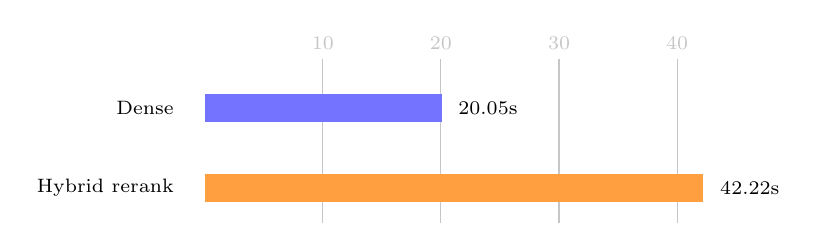
\begin{tikzpicture}[x=0.15cm,y=0.78cm,font=\scriptsize]
\foreach \x in {10,20,30,40}
  \draw[gray!45] (\x,0.48) -- (\x,3.15) node[above]{\x};

\node[anchor=east] at (-1.8,2.35) {Dense};
\fill[blue!55] (0,2.12) rectangle (20.05,2.58);
\node[anchor=west] at (20.65,2.35) {20.05s};

\node[anchor=east] at (-1.8,1.05) {Hybrid rerank};
\fill[orange!75] (0,0.82) rectangle (42.22,1.28);
\node[anchor=west] at (42.82,1.05) {42.22s};
\end{tikzpicture}
}
\caption{Mean end-to-end latency for the measured pilot run, including retrieval and generation. Blue indicates dense retrieval and orange indicates hybrid rerank. Hybrid rerank was slower primarily because retrieval and reranking dominate the runtime.}
\label{fig:latency}
\end{figure}
